% Template for EUSIPCO-2012 paper; to be used with:
%          spconf.sty  - LaTeX style file, and
%          IEEEbib.bst - IEEE bibliography style file.
% --------------------------------------------------------------------------
\documentclass{article}
\usepackage{balance}
\usepackage{spconf,amsmath,graphicx}
\usepackage{tikz}
\usepackage{amsmath}
\usetikzlibrary{calc,snakes}
\usetikzlibrary{shapes,snakes}
\usetikzlibrary{calc,chains,positioning}
\usepackage{cases}
\usepackage{phaistos}
\usepackage{setspace}
%%%%%\usepackage{flushend}

% Example definitions.
% --------------------
\def\x{{\mathbf x}}
\def\L{{\cal L}}
\ninept
%\def\baselinestretch{1.0}

% Title.
% ------
\title{Non-intrusive Regularization for Least-Squares Multichannel Equalization for Speech Dereverberation}
%
% Single address.
% ---------------
\name{Ina Kodrasi, Simon Doclo}
\address{
%email of first author
%affiliation and address of first author
University of Oldenburg, Institute of Physics, Signal Processing Group, Oldenburg, Germany \\
{\tt \char123 ina.kodrasi,simon.doclo\char125 @uni-oldenburg.de}\\
%affiliations of remaining authors
}


\begin{document}

\maketitle
%
\begin{abstract}
Multichannel equalization techniques for speech dereverberation are known to be highly sensitive to errors arising during the identification of the room impulse responses. 
In order to increase their robustness, it has been proposed to incorporate regularization. 
However, the optimal regularization parameter yielding the highest perceptual sound quality has generally been determined intrusively, limiting the practical applicability. 

In this paper, we propose an automatic and non-intrusive selection procedure for the regularization parameter based on the L-curve and extensively investigate its performance. 
Experimental results show that using the automatic regularization procedure for a recently proposed partial multichannel equalization technique (P-MINT) leads to a very similar performance as using the intrusively determined optimal regularization parameter. 
Furthermore, it is shown that the automatically regularized P-MINT technique outperforms state-of-the-art multichannel equalization techniques such as channel shortening and relaxed multichannel least-squares, both in terms of reverberant tail suppression and perceptual sound quality (PESQ).
\end{abstract}

\begin{keywords}
acoustic multichannel equalization, speech dereverberation, automatic regularization
\end{keywords}
%


\section{Introduction}
\label{sec: intro}
In many hands-free telecommunication applications the recorded microphone signals are often corrupted by reverberation, which typically degrades the quality of the speech signals, impairs speech intelligibility, and decreases the performance of automatic speech recognition systems. 
In order to mitigate these detrimental effects of reverberation several dereverberation approaches have been investigated in the past decades~\cite{Naylor_Derev_book}.
One particular class of speech dereverberation approaches is acoustic multichannel equalization~\cite{Miyoshi_ITASS_1988, Kallinger_ICASSP_2006, Zhang_IWAENC_2010, Kodrasi_ICASSP_2012}, which is based on designing filters to reshape the estimated room impulse responses~(RIRs) between the source and the microphone array.

The well-known multiple-input/output inverse theorem~(MINT) \cite{Miyoshi_ITASS_1988} can achieve in theory the highest dereverberation performance and recover the anechoic speech signal, making acoustic multichannel equalization a very attractive approach to speech dereverberation.
However, since the estimated RIRs generally differ from the real ones~(e.g. due to the sensitivity of blind system identification methods to interfering noise~\cite{Hasan_EUSIPCO_2006}), MINT fails to equalize the true RIRs and typically yields large distortions in the processed output signal~\cite{Radlovic_ITSA_2000}.
Aiming at increasing robustness to estimation errors by relaxing the constraints on the filter design, partial multichannel equalization techniques such as channel shortening~(CS)~\cite{Kallinger_ICASSP_2006} and relaxed multichannel least-squares~(RMCLS)~\cite{Zhang_IWAENC_2010} have been investigated. 
Since late reverberation (typically defined as the part of the RIR after $50$-$80$ ms) is the main cause of sound quality degradation~\cite{}, such techniques aim at suppressing only the reverberant tail without constraining the early reflections, which might however lead to undesired perceptual effects.

In order to directly control the perceptual speech quality, a partial multichannel equalization technique based on MINT~(P-MINT) has been recently proposed~\cite{Kodrasi_ICASSP_2012}.
To further increase its robustness, regularization has been incorporated.
However, in order to select an optimal regularization parameter that leads to a high perceptual quality, an intrusive procedure requiring knowledge of the true RIRs has been employed, limiting the application of the regularized P-MINT technique in practice.

In this paper, we propose an automatic and non-intrusive selection procedure for the regularization parameter based on the L-curve criterion~\cite{Hansen_1993} and thoroughly investigate its performance.
This non-intrusive procedure is discussed for the regularized P-MINT technique since it has been shown in~\cite{Kodrasi_ICASSP_2012} that regularized P-MINT outperforms state-of-the-art techniques such as RMCLS and CS.
However, the procedure proposed here can be extended to any regularized least-squares multichannel equalization technique~(e.g. MINT).
\section{Acoustic Multichannel Equalization}
\label{sec: ame}
Fig.~\ref{fig: acsys} depicts an acoustic system with a single source and $M$ microphones.
The $m$-th microphone signal, $m=1, \; \ldots, \; M$, at time index $n$ is given by $x_m(n) = h_m(n) \ast s(n)$, where~$\ast$ denotes the convolution operation, $s(n)$ is the clean speech signal, and $h_m(n)$ denotes the room impulse response between the source and the $m$-th microphone, which can be described in vector notation as $\mathbf{h}_m = \left[h_m(0) \; h_m(1) \; \ldots \; h_m(L_h-1) \right]^T$, with $L_h$ the RIR length and $[\cdot]^T$ the transpose operation.
\begin{figure}[b!]
  \centering
  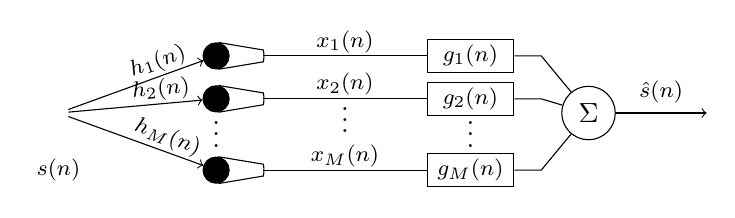
\begin{tikzpicture}
    % Adjustments
    \def\micd{.1cm}                % mic diameter
    \def\micl{.6cm}                % mic length
    \def\micw{.15cm}                % mic width
    \def\micbend{10}               % mic bottom bend
    \def\micdistance{.2cm}         % distance between microphones
    \def\filterdistance{2.5cm}     % distance between microphone and filter
    \def\filteroutline{.9cm}       % length of line which gets out of filter
    \def\sumdistance{1.5cm}        % distance of sum node to the filter
    \def\sumoutline{1cm}           % length of line which gets out of sum
    \def\headdistance{2cm}         % distance between microphone and head

    % Styles
    \tikzset{%
      mic head/.style={fill=black,draw=black,circle,minimum size=\micd},
      filter/.style={draw,minimum width=1.1cm,inner sep=2pt},
      sum/.style={draw,circle},
      xlabel/.style={inner sep=1pt,above,midway},
      sumlabel/.style={xlabel},
      hlabel/.style={xlabel,sloped,pos=.7},
      head/.style={font=\Large}
    }

    % Draw Microphones
    \begin{scope}[start chain=going below,every node/.style={on chain},node distance=\micdistance]
      \node[mic head] (mic1) {};
      \node[mic head] (mic2) {};
      \node[mic head,yshift=-1.8*\micdistance] (mic3) {};
    \end{scope}
    \node[yshift=3pt] at ($(mic2)!.5!(mic3)$) {$\vdots$};

    \foreach \m in {1,2,3} {%
      \coordinate (m1) at ($(mic\m)+(\micl,\micw/2)$);
      \coordinate (m2) at ($(mic\m)+(\micl,-\micw/2)$);
      \draw (tangent cs:node=mic\m,point={(m1)},solution=1) -- (m1) to[bend left=\micbend] (m2) -- (tangent cs:node=mic\m,point={(m2)},solution=2);
    }

    % Draw Filter
    \foreach \m/\i in {1/1,2/2,3/M} {%
      \node[filter,right=\filterdistance of mic\m] (filter\m) {\footnotesize $g_{\i}(n)$};
      \draw ($(mic\m)+(\micl,0)$) to node[xlabel] (x\m) {\footnotesize $x_{\i}(n)$} (filter\m);
    }
    \node[yshift=3pt] at ($(filter2)!.5!(filter3)$) {$\vdots$};
    \node[yshift=3pt] at ($(x2)!.5!(x3)$) {$\vdots$};
    % Sum Node
    \node[sum] (sum) at ($(filter1)!.5!(filter3)+(\sumdistance,0)$) {$\Sigma$};
    \draw[->] (sum) -- node[above] {\footnotesize $\hat{s}(n)$} ++(1.5,0);
    % Connect filter with sum
    \foreach \m in {1,2,3} {%
      \draw (filter\m) -- ++(\filteroutline,0) -- (sum);
    }

    % Head
    \node[head] (head) at ($(mic1)!.5!(mic3)-(\headdistance,0)$) {\PHtattooedHead};
    \node[fill=white,minimum width=4.8pt,minimum height=5.7pt,inner sep=0pt] at ($(head.center)+(2.3pt,-2.5pt)$) {};
    \node at ($(head.center)+(0.0pt,-20.5pt)$) {\footnotesize $s(n)$};
    % Connect head with mics
    \foreach \m/\i in {1/1,2/2,3/M} {%
      \draw[->] (head) -- node[hlabel] {\footnotesize $h_{\i}(n)$} (mic\m);
    }
  \end{tikzpicture}
  \caption{Multichannel equalization system}
  \label{fig: acsys}
\end{figure}
Applying filters $g_m(n)$ of length $L_g$, i.e. $\mathbf{g}_m = \left[g_m(0) \; g_m(1) \; \ldots \; g_m(L_g-1) \right]^T$, the output signal $\hat{s}(n)$ of the multichannel equalization system is given by the sum of the filtered microphone signals, i.e.
\begin{align}
  \hat{s}(n) & = \sum_{m=1}^{M} x_m(n) \ast g_m(n) \\
  & = s(n) \ast \underbrace{\sum_{m=1}^{M} h_m(n) \ast g_m(n)}_{c(n)} = s(n) \ast c(n),
\end{align}
where $c(n)$ is the equalized impulse response~(EIR) between the source and the output of the system, which can be described in vector notation as $\mathbf{c} = \left[c(0) \; c(1) \; \ldots \; c(L_c-1)\right]^T$, with $L_c = L_h+L_g-1$.
Using the $ML_g$--dimensional stacked filter vector $\mathbf{g}$ and the $L_c \times ML_g$--dimensional multichannel convolution matrix $\mathbf{H}$, i.e.
\begin{align}
  \mathbf{g}  &=  \left[\mathbf{g}_1^T \; \mathbf{g}_2^T \; \ldots \; \mathbf{g}_M^T \right]^T \\
  \mathbf{H}  &= \left[\mathbf{H}_1 \; \mathbf{H}_2 \; \ldots \; \mathbf{H}_M \right],
\end{align}
with $\mathbf{H}_m$ the $L_c \times L_g$--dimensional convolution matrix of $\mathbf{h}_m$, the EIR can be expressed as
\begin{equation}
\label{eq: eir}
\boxed{\mathbf{c} = \mathbf{H}\mathbf{g}}
\end{equation}
The filters $\mathbf{g}$ can then be constructed based on different design objectives for $\mathbf{c}$.

However, the estimated RIRs $\hat{\mathbf{h}}_m$ typically differ from the real ones and hence, the estimated multichannel convolution matrix $\hat{\mathbf{H}}$ differs from $\mathbf{H}$. 
Therefore in practice techniques such as the ones described in the following design filters $\mathbf{g}$ to optimize the estimated EIR $\hat{\mathbf{c}} = \hat{\mathbf{H}}\mathbf{g}$.

\smallskip \noindent \textit{MINT.} \enspace
The multiple-input/output inverse theorem~\cite{Miyoshi_ITASS_1988} aims to exactly invert the system up to a desired delay $\tau$ by designing inverse filters $\mathbf{g}$ such that $\hat{\mathbf{H}}\mathbf{g} = \mathbf{d}$, where $\mathbf{d}$ is the desired EIR defined as a delayed impulse, i.e. $\mathbf{d} = [\underbrace{0 \; \ldots \; 0}_{\tau} \; 1 \; 0 \; \ldots \; 0 ]^T$.
Inverse filters are then computed by minimizing the least-squares cost function
\begin{equation}
\label{eq: ls}
\boxed{J_{_{\rm MINT}}(\mathbf{g}) = \|\hat{\mathbf{H}}\mathbf{g} - \mathbf{d}\|_2^2}
\end{equation}
It has been shown in~\cite{Miyoshi_ITASS_1988} that when the RIRs do not share any common zeros and when $L_g \geq \lceil{\frac{L_h-1}{M-1}\rceil}$, filters that invert the multichannel acoustic system can be computed as
\begin{equation}
  \label{eq: mint}
  \boxed{\mathbf{g}_{{}_{\rm MINT}} = \hat{\mathbf{H}}^+\mathbf{d}}
\end{equation}
with $\{\cdot\}^+$ denoting the Moore-Penrose pseudo-inverse. Since the matrix $\hat{\mathbf{H}}$ is a full row-rank matrix~\cite{Harikumar_ITSP_1998}, its pseudo-inverse can be computed as $\hat{\mathbf{H}}^+ = \hat{\mathbf{H}}^T(\hat{\mathbf{H}}\hat{\mathbf{H}}^T)^{-1}$.
However, such a technique is very sensitive to RIR estimation errors, leading to an equalized impulse response $\mathbf{c} = \mathbf{H}\hat{\mathbf{H}}^+\mathbf{d} \neq \mathbf{d}$ which typically causes large distortions in the output signal.
Experimental investigations in~\cite{Zhang_IWAENC_2010, Kodrasi_ICASSP_2012} have shown that techniques aiming only at partial equalization such as partial multichannel equalization approach based on MINT\footnote{For an overview of other partial multichannel equalization techniques such as CS and RMCLS the reader is referred to~\cite{Kallinger_ICASSP_2006, Zhang_IWAENC_2010, Kodrasi_ICASSP_2012}.} are significantly more robust.

\smallskip \noindent \textit{P-MINT.} \enspace
The partial multichannel equalization approach based on MINT~\cite{Kodrasi_ICASSP_2012} aims at setting the reverberant tail of the EIR to $0$, while still controlling the remaining taps corresponding to the direct path and early reflections. 
To accomplish this objective, the first part of one of the estimated RIRs is used as the target response in~(\ref{eq: ls}), i.e.  
\begin{equation}
\boxed{J_{{}_{\rm P-MINT}}(\mathbf{g}) = \|{\hat{\mathbf{H}}}\mathbf{g} - {\hat{\mathbf{h}}}_p^{\rm d}\|_2^2}
\end{equation}
where
\begin{equation}
\hat{\mathbf{h}}_{p}^{\rm d} = [\underbrace{0\phantom{\rlap{$(L_d-1)$}} \ldots 0 }_{\tau} \underbrace{\hat{h}_p(0) \ldots \hat{h}_p(L_d-1)}_{L_d} 0 \ldots 0 ]^{T},
\end{equation}
with $p \in \{1, \; \ldots, \; M\}$ and $L_d$ denoting the length in number of samples of the direct path and early reflections.
Filters that partially equalize the system can then be computed as
\begin{equation}  
\label{eq: pmintsol}  
\boxed{\mathbf{g}_{{}_{\rm P-MINT}} = {\hat{\mathbf{H}}}^{+}{\hat{\mathbf{h}}}_p^{\rm d}}
\end{equation}  
In order to further increase the robustness of P-MINT to estimation errors, regularization has been incorporated such that the energy of the reshaping filters is decreased.

\smallskip \noindent \textit{Regularized P-MINT.} \enspace In the regularized P-MINT approach in~\cite{Kodrasi_ICASSP_2012}, the P-MINT cost function is extended to
\begin{equation}
\label{eq: cost_rpmint}
\boxed{J_{{}_{\rm P-MINT}}^{^{_{\rm R}}}(\mathbf{g}) = \|\hat{\mathbf{H}}\mathbf{g} - \hat{\mathbf{h}}_p^{\rm d}\|_2^2 + \delta \|\mathbf{g} \|_2^2}
\end{equation}
with $\delta$ a regularization parameter controlling the weight given to the minimization of the energy of $\mathbf{g}$.
The regularized P-MINT filters minimizing~(\ref{eq: cost_rpmint}) can then be calculated as
\begin{equation}
\label{eq: rpmintsol}
\boxed{\mathbf{g}_{{}_{\rm P-MINT}}^{_{\rm R}}  = (\hat{\mathbf{H}}^T\hat{\mathbf{H}}+\delta \mathbf{I})^{-1}\hat{\mathbf{H}}^{T}\hat{\mathbf{h}}_p^{\rm d}}
\end{equation}
where $\mathbf{I}$ is the $ML_g \times ML_g$--dimensional identity matrix.

Increasing the value of the regularization parameter $\delta$ decreases the energy of $\mathbf{g}$, making the reshaping filters less sensitive to errors in the estimated RIRs. 
However, increasing this parameter also reduces the equalization performance with respect to the true RIRs, resulting in a trade-off between performance for perfectly estimated room impulse responses and robustness in the presence of estimation errors.

\section{Non-intrusive Selection of the Regularization Parameter}
Clearly different values of the regularization parameter $\delta$ in~(\ref{eq: rpmintsol}) yield different reshaping filters $\mathbf{g}$ which lead to different performance. 
The optimal regularization parameter $\delta_{\rm opt}$ that yields the highest perceptual sound quality differs depending on the acoustic system to be equalized and the system estimation errors. 
In~\cite{Kodrasi_ICASSP_2012}, $\delta_{\rm opt}$ has been intrusively determined by using the true room impulse responses~(cf. Section~\ref{sec: exp}), which are however unknown in practice.
Hence an automatic and non-intrusive procedure for the selection of the regularization parameter is required.

The cost function in~(\ref{eq: cost_rpmint}) shows that integrating regularization introduces a trade-off between minimizing the residual energy $\|\hat{\mathbf{H}}\mathbf{g}_{{}_{\rm P-MINT}}^{_{\rm R}} - \hat{\mathbf{h}}_p^{\rm d}\|_2^2$ and minimizing the filter energy $\|\mathbf{g}_{{}_{\rm P-MINT}}^{_{\rm R}}\|_2^2$.
In order to automatically compute a regularization parameter $\delta_{\rm auto}$ that keeps both of these quantities small, it has been proposed in~\cite{Hansen_1993} to use a parametric plot of the filter norm versus the residual norm for several values of $\delta$.
This plot always has an L-shape with the corner located exactly where the reshaping filter changes in nature from being dominated by over-regularization to being dominated by under-regularization. 
We propose selecting the regularization parameter $\delta_{\rm auto}$ in the regularized P-MINT technique as the one corresponding to the corner of the parametric plot of $\|\mathbf{g}_{{}_{\rm P-MINT}}^{_{\rm R}}\|_2$ versus $\|\hat{\mathbf{H}}\mathbf{g}_{{}_{\rm P-MINT}}^{_{\rm R}} - \hat{\mathbf{h}}_p^{\rm d}\|_2$~(i.e. the point of maximum curvature). 
As it is experimentally validated in Section~\ref{sec: exp}, such a regularization parameter also leads to a nearly optimal perceptual sound quality as $\delta_{\rm opt}$.

The L-curve could be generated by initially computing the reshaping filters $\mathbf{g}_{{}_{\rm P-MINT}}^{_{\rm R}}$ using~(\ref{eq: rpmintsol}) for several regularization parameter values $\delta$ and then calculating the required norms.
However, in order to avoid any significant computational overhead, the L-curve is generated using the singular value decomposition~(SVD) of the estimated convolution matrix $\hat{\mathbf{H}}$ as following.

Consider the SVD of $\hat{\mathbf{H}}$, i.e.
\begin{equation}
\label{eq: svd}
  \hat{\mathbf{H}} = \hat{\mathbf{U}}\hat{\mathbf{S}}\hat{\mathbf{V}}^T,
\end{equation}
where $\hat{\mathbf{U}}$ and $\hat{\mathbf{V}}$ are orthogonal matrices and $\hat{\mathbf{S}}$ is a diagonal matrix consisting of the singular values $\hat{\sigma}_n$ of $\hat{\mathbf{H}}$ in desending order, i.e. $\hat{\mathbf{S}} = {\rm diag}\{\left[\hat{\sigma}_0 \; \hat{\sigma}_1 \; \ldots \; \hat{\sigma}_{L_c-1}\right]\}$. Using~(\ref{eq: rpmintsol}) and~(\ref{eq: svd}), the regularized P-MINT filters can be expressed as
\begin{equation}
\mathbf{g}_{{}_{\rm P-MINT}}^{_{\rm R}}  =  \sum_{n=0}^{L_c-1} \frac{\hat{\sigma}_n \hat{\mathbf{u}}_n^T \hat{\mathbf{h}}_p^{\rm d} }{\hat{\sigma}_n^2+\delta}  \hat{\mathbf{v}}_n,
\end{equation}
where $\hat{\mathbf{u}}_n$ and $\hat{\mathbf{v}}_n$ denote the $n$-th column of $\hat{\mathbf{U}}$ and $\hat{\mathbf{V}}$ respectively.
Hence the inverse filter norm for a given $\delta$ can be computed as
\begin{equation}
\label{eq: eta}
\boxed{\|\mathbf{g}_{{}_{\rm P-MINT}}^{_{\rm R}}\|_2 = \sqrt{\sum_{n = 0}^{L_c-1} \frac{\hat{\sigma}_n^2 (\hat{\mathbf{u}}_n^T \hat{\mathbf{h}}_p^{\rm d})^2}{(\hat{\sigma}_n^2 + \delta)^2}}}
\end{equation}
Furthermore, expressing the norm of the residual as a function of the regularization parameter and of the singular values leads to
\begin{equation}
\label{eq: rho}
\boxed{ \|\hat{\mathbf{H}}\mathbf{g}_{{}_{\rm P-MINT}}^{_{\rm R}} - \hat{\mathbf{h}}_p^{\rm d}\|_2 = \sqrt{\sum_{n = 0}^{L_c-1} \frac{\delta^2 (\hat{\mathbf{u}}_n^T \hat{\mathbf{h}}_p^{\rm d})^2}{(\hat{\sigma}_n^2 + \delta)^2}}}
\end{equation}
Therefore once the SVD is computed, the L-curve can be readily generated using~(\ref{eq: eta}) and~(\ref{eq: rho}).
\begin{figure}[t!]
\centering
\includegraphics[scale = 0.6]{Plots/lcurve_ex}
\caption{Typical L-curve obtained using regularized P-MINT for an erroneously estimated acoustic system}
\label{fig: lcurveex}
\end{figure}

Fig.~\ref{fig: lcurveex} depicts a typical L-curve obtained using regularized P-MINT for equalizing an erroneously estimated acoustic system. 
As illustrated in this figure, increasing the value of $\delta$ decreases the norm of the reshaping filter but at the same time increases the norm of the residual.
Although from such a curve it seems intuitively easy to determine $\delta_{\rm auto}$ that corresponds to the maximum curvature, a numerically stable algorithm is needed to detect it automatically. 
In this work, the triangle method~\cite{Castellanos_2002} is used for locating $\delta_{\rm auto}$.


\section{Experimental Results}
\label{sec: exp}
The performance of the regularized P-MINT technique using the automatic and non-intrusive selection procedure for the regularization parameter is evaluated using a measured acoustic system with $M=2$ and reverberation time $T_{60} = 600$~ms as the true system to be equalized. 
The sampling frequency used is $f_s = 16$~kHz and the simulation parameters are set to $L_h = 2000$, $L_g = 1999$, $\tau = 0$, and $L_d \in \{0.01 f_s, \; 0.02f_s, \; 0.03f_s, \; 0.04f_s, \; 0.05f_s\}$.
To generate the estimated acoustic system, the real RIRs are perturbed by adding scaled white noise as proposed in~\cite{Cho_ITSA_1999}, i.e. $\hat{h}_m(n) = h_m(n) + \epsilon_m(n)$, where $\epsilon_m(n)$ is an uncorrelated Gaussian noise sequence with zero mean and an appropriate variance, such that a \emph{normalized channel mismatch} $E_m$ defined as
\begin{equation}
E_m = 10 \log_{10} \frac{\|\mathbf{h}_m - \hat{\mathbf{h}}_m \|_2^2}{\|\mathbf{h}_m\|_2^2},
\end{equation}
is generated. 
The considered normalized channel mismatch values are 
\begin{equation}
\small
E_m \in \{ -33~{\rm dB}, \; -30~{\rm dB}, \; -25~{\rm dB}, \; -20~{\rm dB}, \; -15~{\rm dB} \}.
\end{equation}
Furthermore, the target response in P-MINT is chosen as the direct path and early reflections of the first estimated channel, i.e. $\hat{\mathbf{h}}_1^{\rm d}$.

The reverberant tail suppression is evaluated using the \emph{energy decay curve}~(EDC) of the obtained EIR $\mathbf{c} = \mathbf{H} \mathbf{g}$, which is defined as
\begin{equation}
\small
\hbox{EDC}(n) = 10 \log_{10}\frac{1}{\|\mathbf{c}\|_2^2}\sum_{i=n}^{L_c-1}c^2(i), \; n = 0,  \ldots,  L_c-1.
\end{equation}
To evaluate the perceptual sound quality we have used the objective speech quality measure PESQ~\cite{PESQ} with $s(n) \ast h_1^{\rm d}(n)$ as reference signal.
It has been shown in~\cite{Goetze_AES_2010} that measures relying on auditory models such as PESQ exhibit the highest correlation with subjective listening tests when evaluating the quality of dereverberated speech.

In order to determine the regularization parameter to be used, we have considered several regularization parameters, i.e. 
\begin{equation}
\label{eq: delta}
 \delta \in \{10^{-9}, \;10^{-8}, \;  \ldots, \; 10^{-1} \}.
\end{equation}
To determine the optimal regularization parameter $\delta_{\rm opt}$, reshaping filters $\mathbf{g}$ have been computed for each $\delta$ in~(\ref{eq: delta}) and the perceptual quality obtained by the EIR they yield, i.e. $\mathbf{c} = \mathbf{H}\mathbf{g}$ has been calculated.
The optimal parameter $\delta_{\rm opt}$ in each scenario is then intrusively selected as the one leading to the highest perceptual sound quality, i.e. PESQ score. 
Furthermore, the automatic parameter $\delta_{\rm auto}$ is selected as the one corresponding to the corner of the L-curve generated with the regularization parameters in~(\ref{eq: delta}).
For the sake of clarity and in order to avoid overcrowded plots this experimental part is structured into two parts. 
\begin{figure}[t!]
\centering
\includegraphics[scale = 0.6]{Plots/EDC_optauto_5_Cm_-33_Ld_800}
\caption{EDC of the EIR obtained using regularized P-MINT with $\delta_{\rm opt}$, regularized P-MINT with $\delta_{\rm auto}$, and EDC of $\mathbf{h}_1$ for the normalized channel mismatch $E_m = -33$~dB and the desired window length $L_d = 0.05f_s$ (i.e. $50$~ms)}
\label{fig: edcoptauto}
\end{figure}

\smallskip \noindent \textit{Experiment 1.} \enspace
In the first experiment, the performance of the regularized P-MINT technique when using $\delta_{\rm auto}$ is compared to the performance when $\delta_{\rm opt}$ is used. 
Fig.~\ref{fig: edcoptauto} depicts the obtained EDCs for the normalized channel mismatch $-33$~dB and the desired window length $50$~ms. 
As can be observed in this figure, the automatic regularization parameter yields a very similar reverberant tail suppression as the optimal regularization parameter, with the reverberant tail being below audible levels.
In order to evaluate the perceptual speech quality that the non-intrusive regularization procedure yields, Fig.~\ref{fig: pesqoptauto}~(a) depicts the PESQ scores of the output $\hat{s}(n)$ obtained using regularized P-MINT with $\delta_{\rm opt}$ and regularized P-MINT with $\delta_{auto}$ for the normalized channel mismatch $E_m = -33$~dB and several desired window lengths.
As illustrated in this figure, the perceptual speech quality when using $\delta_{\rm auto}$ is generally similar to the one obtained when using $\delta_{\rm opt}$, except for the desired window length of $40$~ms where the PESQ score is reduced by approximately $0.5$. 
However, the average PESQ score reduction over all desired window lengths is only $0.2$, implying that as $L_d$ changes as a design parameter, the automatic selection procedure for the regularization parameter yields a nearly optimal performance. 

Since the optimal regularization parameter typically changes as the channel mismatch changes (larger estimation errors in the RIRs require larger regularization), it is important to evaluate the perceptual quality when $\delta_{\rm auto}$ is used for larger normalized channel mismatches.
Fig.~\ref{fig: pesqoptauto}~(b) depicts the PESQ scores obtained using regularized P-MINT with $\delta_{\rm opt}$ and regularized P-MINT with $\delta_{auto}$ for the desired window length $50$~ms and several normalized channel mismatches.
It can be seen that using the automatically computed regularization parameter yields a very similar perceptual quality as $\delta_{\rm opt}$, with an insignificant average performance reduction over all considered $E_m$ of $0.03$.

\smallskip \noindent \textit{Experiment 2.} \enspace
In this experimental part, the performance of the regularized P-MINT technique when using $\delta_{\rm auto}$ is compared to the performance of state-of-the-art techniques such as CS and RMCLS.
Fig.~\ref{fig: edcall} depicts the EDCs obtained for the normalized channel mismatch $-33$~dB and the desired window length $50$~ms. 
As illustrated in this figure MINT fails to invert the channel, leading to an EDC that is even higher than the one of the original RIR. 
Furthermore, also the channel shortening technique fails to reshape the channel, yielding an audible reverberant tail.
On the other hand, the RMCLS and the automatically regularized P-MINT techniques are significantly more robust, with RMCLS yielding the highest reverberant tail suppression.
However, since the EDC does not fully describe the quality of the processed speech, it is important to evaluate whether RMCLS also yields the highest PESQ score.
Fig.~\ref{fig: pesqall}~(a) depicts the obtained PESQ scores for several desired window lengths and $E_m = -33$~dB.
As illutrated in this figure, the regularized P-MINT approach using the automatic non-intrusive regularization procedure outperforms MINT, CS, as well as RMCLS for the desired window lengths $30$~ms, $40$~ms, and $50$~ms, whereas similar performance as RMCLS is achieved for $10$~ms and $20$~ms.
Furthermore, Fig.~\ref{fig: pesqall}~(b) illustrates the obtained PESQ scores for $L_d = 0.05 f_s$~(i.e. $50$~ms) and several normalized channel mismatch values.
It can be seen that the automatically regularized P-MINT technique yields a significantly higher perceptual speech quality than all other state-of-the-art techniques for all considered normalized channel mismatch values. 

The results presented in these simulations show that the automatic selection procedure for the regularization parameter yields a nearly optimal perceptual sound quality in the regularized P-MINT approach. 
Furthermore, it is shown that the automatically regularized P-MINT technique always yields a similar or higher performance than other state-of-the-art equalization techniques.
% making regularized P-MINT a robust, perceptually advantageous, and practically applicable multichannel equalization technique for speech dereverberation.
\begin{figure}[t!]
\centering
\includegraphics[scale = 0.6]{Plots/PESQ_optauto_5}

\hspace{0.7cm} (a) \hspace{3.3cm} (b)
\caption{PESQ score of $\hat{s}(n)$ obtained using regularized P-MINT with $\delta_{\rm opt}$, regularized P-MINT with $\delta_{\rm auto}$, and PESQ score of the reverberant signal for (a) normalized channel mismatch $E_m = -33$~dB and several desired window lengths $L_d$ and (b) several normalized channel mismatches $E_m$ and desired window length $L_d = 0.05 f_s$~(i.e. $50$~ms)}
\label{fig: pesqoptauto}
\end{figure}


\section{Conclusion}
In this paper we have presented an automatic and non-intrusive procedure based on the L-curve for selecting the regularization parameter in regularized least-squares acoustic multichannel equalization techniques. 
The performance of this procedure has been extensively investigated and compared to the performance when the intrusively selected optimal regularization parameter is used for the regularized P-MINT technique.
Simulation results show that using the automatically determined regularization parameter yields very similar performance as the optimally determined one. 
Furthermore, it has been shown that the regularized P-MINT approach using the automatically determined regularization parameter outperforms state-of-the-art techniques such as RMCLS and CS both in terms of reverberant tail suppression and perceptual speech quality.
\begin{figure}[t!]
\centering
\includegraphics[scale = 0.6]{Plots/EDC_all_sys_5_Cm_-33_Ld_800}
\caption{EDC of the EIR obtained using MINT, CS, RMCLS, regularized P-MINT with $\delta_{\rm auto}$, and EDC of $\mathbf{h}_1$ for the normalized channel mismatch $E_m = -33$~dB and the desired window length $L_d = 0.05f_s$ (i.e. $50$~ms)}
\label{fig: edcall}
\end{figure}


% Below is an example of how to insert images. Delete the ``\vspace'' line,
% uncomment the preceding line ``\centerline...'' and replace ``imageX.ps''
% with a suitable PostScript file name.
% -------------------------------------------------------------------------


\bibliographystyle{IEEEtran}
\bibliography{refs}

\begin{figure}[t!]
\centering
\includegraphics[scale = 0.6]{Plots/PESQ_all_5}

\hspace{0.7cm} (a) \hspace{3.3cm} (b)
\caption{PESQ score of $\hat{s}(n)$ obtained using  MINT, CS, RMCLS, regularized P-MINT with $\delta_{\rm auto}$, and PESQ score of the reverberant signal for (a) the normalized channel mismatch $E_m = -33$~dB and several desired window lengths $L_d$ and (b) several normalized channel mismatches $E_m$ and desired window length $L_d = 0.05 f_s$~(i.e. $50$~ms)}
\label{fig: pesqall}
\end{figure}
\balance
\end{document}
